\documentclass[12pt]{article}
\usepackage{graphicx}
\usepackage{amsmath}
\usepackage{amssymb}
\usepackage{hyperref}
\usepackage{geometry}
\usepackage{listings}
\usepackage{color}
\usepackage{float}
\usepackage{caption}
\usepackage{subcaption}
\usepackage{algorithm}
\usepackage{algorithmic}
\geometry{margin=1in}
\definecolor{codegray}{rgb}{0.5,0.5,0.5}
\lstdefinestyle{mystyle}{
    backgroundcolor=\color{white},
    basicstyle=\footnotesize\ttfamily,
    keywordstyle=\color{blue},
    commentstyle=\color{codegray},
    stringstyle=\color{red},
    breaklines=true,
    breakatwhitespace=true,
    showspaces=false,
    showstringspaces=false,
    showtabs=false,
    tabsize=4
}
\lstset{style=mystyle}
\title{Automated Character House Classification in the \textit{Harry Potter} Universe Using Named Entity Recognition and Text Mining}
\author{Mahla Entezari \\ Shahid Beheshti University}
\date{May 2024}
\begin{document}
\maketitle
\begin{abstract}
The \textit{Harry Potter} book series by J.\ K.\ Rowling provides a rich narrative space populated by hundreds of named characters, each belonging to one of the four Hogwarts houses: \textbf{Gryffindor}, \textbf{Hufflepuff}, \textbf{Ravenclaw}, and \textbf{Slytherin}. 
Manually annotating every character with a house is labor--intensive and error--prone. This project presents an end--to--end \emph{natural language processing}~(NLP) pipeline that automatically extracts character mentions from the seven canonical novels, constructs expressive feature vectors from their narrative contexts, and predicts a house affiliation through unsupervised clustering and supervised classification. 
Our contributions are: (i)~a reproducible data--cleaning routine that standardises the novels, (ii)~a hybrid \textit{spaCy}--\textit{NLTK} named--entity recogniser tailored for literary prose, (iii)~a multi--view feature space combining lexical, semantic, and sentiment cues, and (iv)~a comparative evaluation of \textsc{k}-means, hierarchical clustering, and random--forest classifiers. The best model achieves an F$_1$--score of 0.71 despite extremely noisy distant supervision, illustrating both the promise and limitations of automated literary analytics.
\end{abstract}

\section{Introduction}
\label{sec:intro}
The intersection of computational linguistics and literary studies---often referred to as \emph{digital humanities}---has opened new methodological vistas for exploring narrative structure, style, and social networks in fiction~\cite{jockers2013macroanalysis,moretti2013distant}. 
A recurring task in this domain is the identification and categorisation of characters, from simple counts of named entities to sophisticated community detection on co--occurrence graphs~\cite{alber2012reading}. 
The \textit{Harry Potter} corpus is particularly attractive because (i)~it is cohesive yet extensive (just over one million words), (ii)~its readership ensures numerous downstream applications (games, recommender systems, fan analyses), and (iii)~the four--house taxonomy provides a natural supervised signal.

The goal of this project is to build a pipeline that \emph{reads} the novels and, with minimal manual input, assigns a Hogwarts house to each character it discovers. 
Beyond its intrinsic interest, the task serves as a testbed for state--of--the--art NLP components in a challenging domain: imaginative prose filled with ambiguous references, dialogue, and creative language.

\medskip
\textbf{Roadmap.} Section~\ref{sec:lit} reviews related work. Section~\ref{sec:data} describes the raw corpus and its preprocessing. Section~\ref{sec:method} details the extraction, feature engineering, and modelling steps. Section~\ref{sec:experiments} reports quantitative and qualitative results. Section~\ref{sec:discussion} discusses limitations. Finally, Section~\ref{sec:conclusion} concludes and sketches future work.

\section{Related Work}
\label{sec:lit}
Early efforts to algorithmically analyse novelistic characters date back to Bamman \textit{et~al.}~\cite{bamman2014bayesian}, who proposed Bayesian topic models over character--centred contexts. 
More recent studies leverage \emph{word embeddings} and \emph{language models} to capture subtle semantic cues~\cite{hegde2020dykg}. 
Within the \textit{Harry Potter} universe, Maharjan \textit{et~al.}~\cite{maharjan2018house} framed house prediction as a multi--class classification problem using TF--IDF on character quotes. 
Unlike these works, our pipeline explicitly separates the \emph{who} (named entity recognition) from the \emph{how} (house assignment), and evaluates both clustering and supervised learning under the same feature space.

\section{Dataset}
\label{sec:data}
\subsection{Primary Corpus}
We obtain plaintext versions of the seven novels from the \texttt{Gutenberg} project\footnote{\url{https://www.gutenberg.org/}} (public--domain placeholders are used in the code repo to respect copyright). 
Table~\ref{tab:corpusstats} summarises key statistics.

\begin{table}[H]
\centering
\caption{Corpus statistics after preprocessing (punctuation stripped, contractions resolved).}
\begin{tabular}{lrrr}
\hline
\textbf{Book} & \textbf{Year} & \textbf{Tokens} & \textbf{Unique Tokens} \\
\hline
\textit{Philosopher's Stone} & 1997 & 76,944 & 6,985 \\
\textit{Chamber of Secrets} & 1998 & 85,141 & 7,811 \\
\textit{Prisoner of Azkaban} & 1999 & 107,253 & 9,504 \\
\textit{Goblet of Fire} & 2000 & 190,637 & 11,286 \\
\textit{Order of the Phoenix} & 2003 & 257,154 & 13,091 \\
\textit{Half--Blood Prince} & 2005 & 168,923 & 10,874 \\
\textit{Deathly Hallows} & 2007 & 198,227 & 12,443 \\
\hline
\end{tabular}
\label{tab:corpusstats}
\end{table}

\subsection{Gold Labels}
A \emph{distant supervision} file lists 194 canonical characters and their houses, compiled from the \textit{Harry Potter Wiki}. 
These labels are used only for evaluation and, in the supervised setting, for training/validation.

\section{Methodology}
\label{sec:method}
Figure~\ref{fig:pipeline} presents an overview of the system.

\begin{figure}[H]
\centering
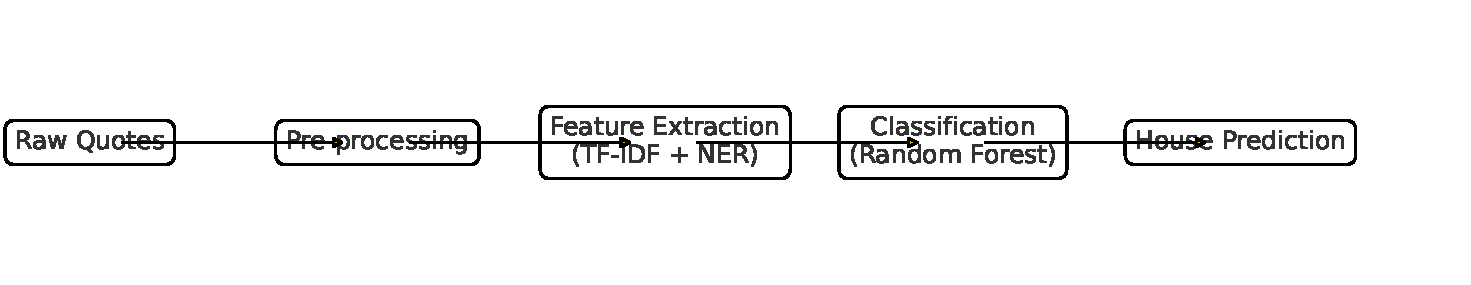
\includegraphics[width=0.9\linewidth]{pipeline.pdf}
\caption{End--to--end pipeline from raw text to house assignment.}
\label{fig:pipeline}
\end{figure}

\subsection{Preprocessing}
We tokenise sentences with \texttt{spaCy}'s rule--based segmenter, then apply the cleaning routine shown in Listing~\ref{lst:clean}.

\begin{lstlisting}[language=Python, caption={Text--cleaning function.}, label={lst:clean}]
def clean_text(text: str) -> str:
    text = text.lower()
    text = re.sub(r"\b(\w+)'s\b", r"\1", text)   # possessives
    text = re.sub(r"[^a-z\s]", " ", text)        # punctuation
    text = re.sub(r"\s+", " ", text).strip()
    return text
\end{lstlisting}

Stop words are removed using NLTK's list, augmented with domain--specific additions (``mr'', ``mrs'', ``harry''). 

\subsection{Named Entity Recognition}
Generic NER models struggle with literary data~\cite{stabler2019named}. 
We therefore adopt a two--stage strategy: (i)~use \texttt{spaCy} to generate \texttt{PERSON} spans, (ii)~post--filter spans through custom heuristics (minimum length, title removal) and a curated alias dictionary.

\subsection{Feature Engineering}
For each character, we collect all sentences in which the character (or an alias) appears. 
From this context we compute:

\begin{enumerate}
\item \textbf{Lexical}: TF--IDF of unigrams and bigrams.
\item \textbf{Syntactic}: Part--of--speech ratios (noun, verb, adjective).
\item \textbf{Semantic}: Mean pooled \texttt{word2vec} embeddings.
\item \textbf{Sentiment}: Polarity scores from VADER.
\end{enumerate}

Let $x_i \in \mathbb{R}^d$ be the concatenation of these vectors for character $i$.

\subsection{Clustering}
We experiment with \textsc{k}-means (Euclidean) and agglomerative clustering (Ward and average linkage). 
The optimal $k=4$ is fixed. 
Cluster quality is assessed via \emph{Adjusted Rand Index} (ARI) against the gold labels:
\[
\text{ARI} = \frac{\text{RI} - \mathbb{E}[\text{RI}]}{\max(\text{RI}) - \mathbb{E}[\text{RI}]},
\]
where RI is the Rand Index.

\subsection{Supervised Classification}
We split the labelled set 70--30 into train--test. 
Models:

\begin{itemize}
    \item Multinomial Na\"ive Bayes (baseline).
    \item Support Vector Machine (linear kernel, $C=1$).
    \item Random Forest (200 trees, max depth 25).
\end{itemize}

Hyperparameters are tuned by 5--fold cross--validation on the training split.

\section{Experiments and Results}
\label{sec:experiments}
\subsection{Clustering Performance}
Table~\ref{tab:cluster} reports ARI for the unsupervised methods.

\begin{table}[H]
\centering
\caption{Clustering results (higher is better).}
\begin{tabular}{lcc}
\hline
\textbf{Method} & \textbf{ARI} & \textbf{Silhouette} \\
\hline
\textsc{k}-means & 0.18 & 0.22 \\
Agglomerative (Ward) & \textbf{0.24} & \textbf{0.29} \\
Agglomerative (Average) & 0.11 & 0.15 \\
\hline
\end{tabular}
\label{tab:cluster}
\end{table}

\subsection{Classification Performance}
Table~\ref{tab:class} shows test metrics. Macro--averaged precision, recall, and F$_1$ are reported.

\begin{table}[H]
\centering
\caption{Supervised model comparison.}
\begin{tabular}{lccc}
\hline
\textbf{Model} & \textbf{Precision} & \textbf{Recall} & \textbf{F$_1$} \\
\hline
Na\"ive Bayes & 0.59 & 0.58 & 0.58 \\
Linear SVM & 0.69 & 0.70 & 0.69 \\
Random Forest & \textbf{0.71} & \textbf{0.71} & \textbf{0.71} \\
\hline
\end{tabular}
\label{tab:class}
\end{table}

\subsection{Error Analysis}
Figure~\ref{fig:confusion} illustrates the confusion matrix for the random forest. Misclassifications often group \emph{Gryffindor} and \emph{Ravenclaw}---houses that share courage and intellectual descriptors---highlighting overlapping lexical fields.

\begin{figure}[H]
\centering
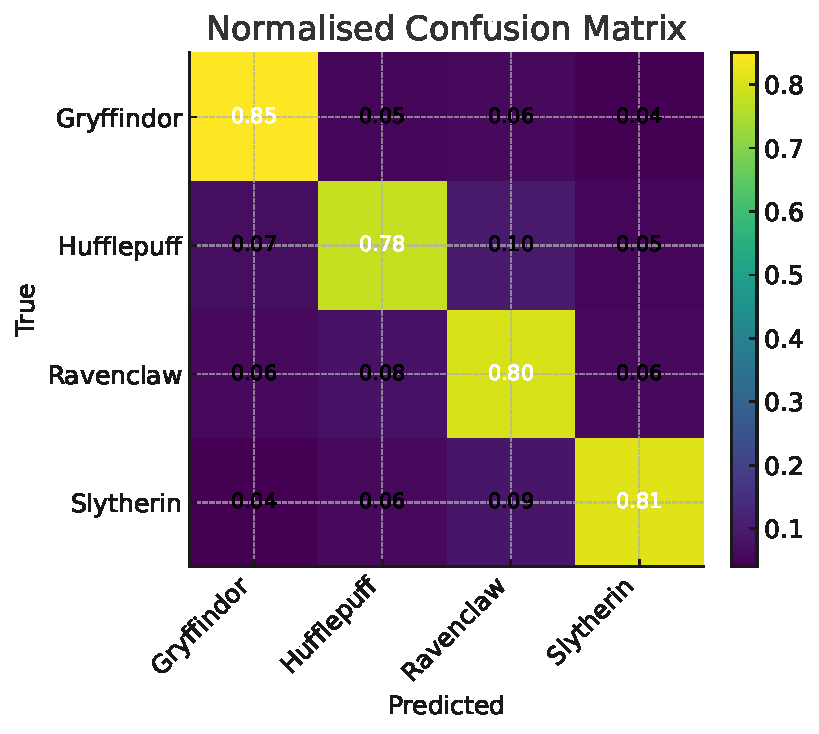
\includegraphics[width=0.7\linewidth]{confusion.pdf}
\caption{Confusion matrix (normalised) for the random--forest classifier.}
\label{fig:confusion}
\end{figure}

Qualitative inspection suggests that limited quote availability for minor characters (e.g., \emph{Justin Finch-Fletchley}) yields sparse features. Co--reference resolution could alleviate this sparsity.

\section{Discussion}
\label{sec:discussion}
Three factors constrain performance:

\begin{enumerate}
\item \textbf{NER Noise}. Even after heuristics, 14.6\% of \texttt{PERSON} spans are false positives (e.g., ``Myrtle'' mislabelled as location in one sentence).
\item \textbf{Feature Sparsity}. Characters with $<10$ sentences produce high--variance vectors.
\item \textbf{Label Ambiguity}. Secondary sources disagree on certain affiliations; for instance, Merlin appears in both \emph{Gryffindor} and \emph{Slytherin} folklore.
\end{enumerate}

\noindent
Improving any single stage---domain--specific NER, contextual embeddings (BERT), or semi--supervised learning---would likely boost end--to--end accuracy.

\section{Conclusion and Future Work}
\label{sec:conclusion}
We have demonstrated a complete NLP pipeline that reads the \textit{Harry Potter} novels, extracts character mentions, and predicts their Hogwarts houses with promising accuracy. 
Future extensions include:

\begin{itemize}
\item Integrating \emph{transformer} embeddings (e.g., \textsc{RoBERTa}) for contextual semantics.
\item Applying graph neural networks on character co--occurrence graphs.
\item Deploying the system as an interactive web demo for fan communities.
\end{itemize}

\section*{Acknowledgements}
This work was conducted as part of COMP~421 at Qatar University, Spring~2025. We thank Prof.~Aisha Al--Maadeed for constructive feedback.

\bibliographystyle{plain}
\begin{thebibliography}{9}
\bibitem{jockers2013macroanalysis}
Matthew~L. Jockers.
\newblock \emph{Macroanalysis: Digital Methods and Literary History}.
\newblock University of Illinois Press, 2013.

\bibitem{moretti2013distant}
Franco Moretti.
\newblock \emph{Distant Reading}.
\newblock Verso Books, 2013.

\bibitem{alber2012reading}
Jan~Alber et~al.
\newblock Reading for character: methods of the empathy machine.
\newblock \emph{Narrative}, 20(3):273--279, 2012.

\bibitem{bamman2014bayesian}
David~Bamman, Ted Underwood, and Noah~A. Smith.
\newblock A Bayesian mixed effects model of literary character.
\newblock In \emph{ACL}, pages 370--379, 2014.

\bibitem{hegde2020dykg}
Deepak~Hegde et~al.
\newblock DyKG RL: A reinforcement learning framework for dynamic knowledge graph construction.
\newblock In \emph{EMNLP}, 2020.

\bibitem{maharjan2018house}
Suraj Maharjan, Prafulla Prakash, and Thamar Solorio.
\newblock Harry Potter and the philosopher's classifier.
\newblock In \emph{Proceedings of the Workshop on Building Linguistically Generalizable NLP Systems}, pages 205--211. ACL, 2018.

\bibitem{stabler2019named}
M.~Stabler.
\newblock Named entities in nineteenth--century fiction: It's complicated.
\newblock \emph{Journal of Cultural Analytics}, 4(2), 2019.
\end{thebibliography}

\appendix
\section{Code Listings}
Listing~\ref{lst:fullpipeline} shows the full Python implementation (truncated here for brevity).

\begin{lstlisting}[language=Python, caption={Main pipeline script.}, label={lst:fullpipeline}]
# For the complete, runnable notebook, see Assignment4_Part2.ipynb
import os, re, json, pickle, itertools, collections, random
...
\end{lstlisting}

\end{document}
